\chapter{Use Case Definition - Connected Cabin System}

\begin{figure}
	\begin{center}
		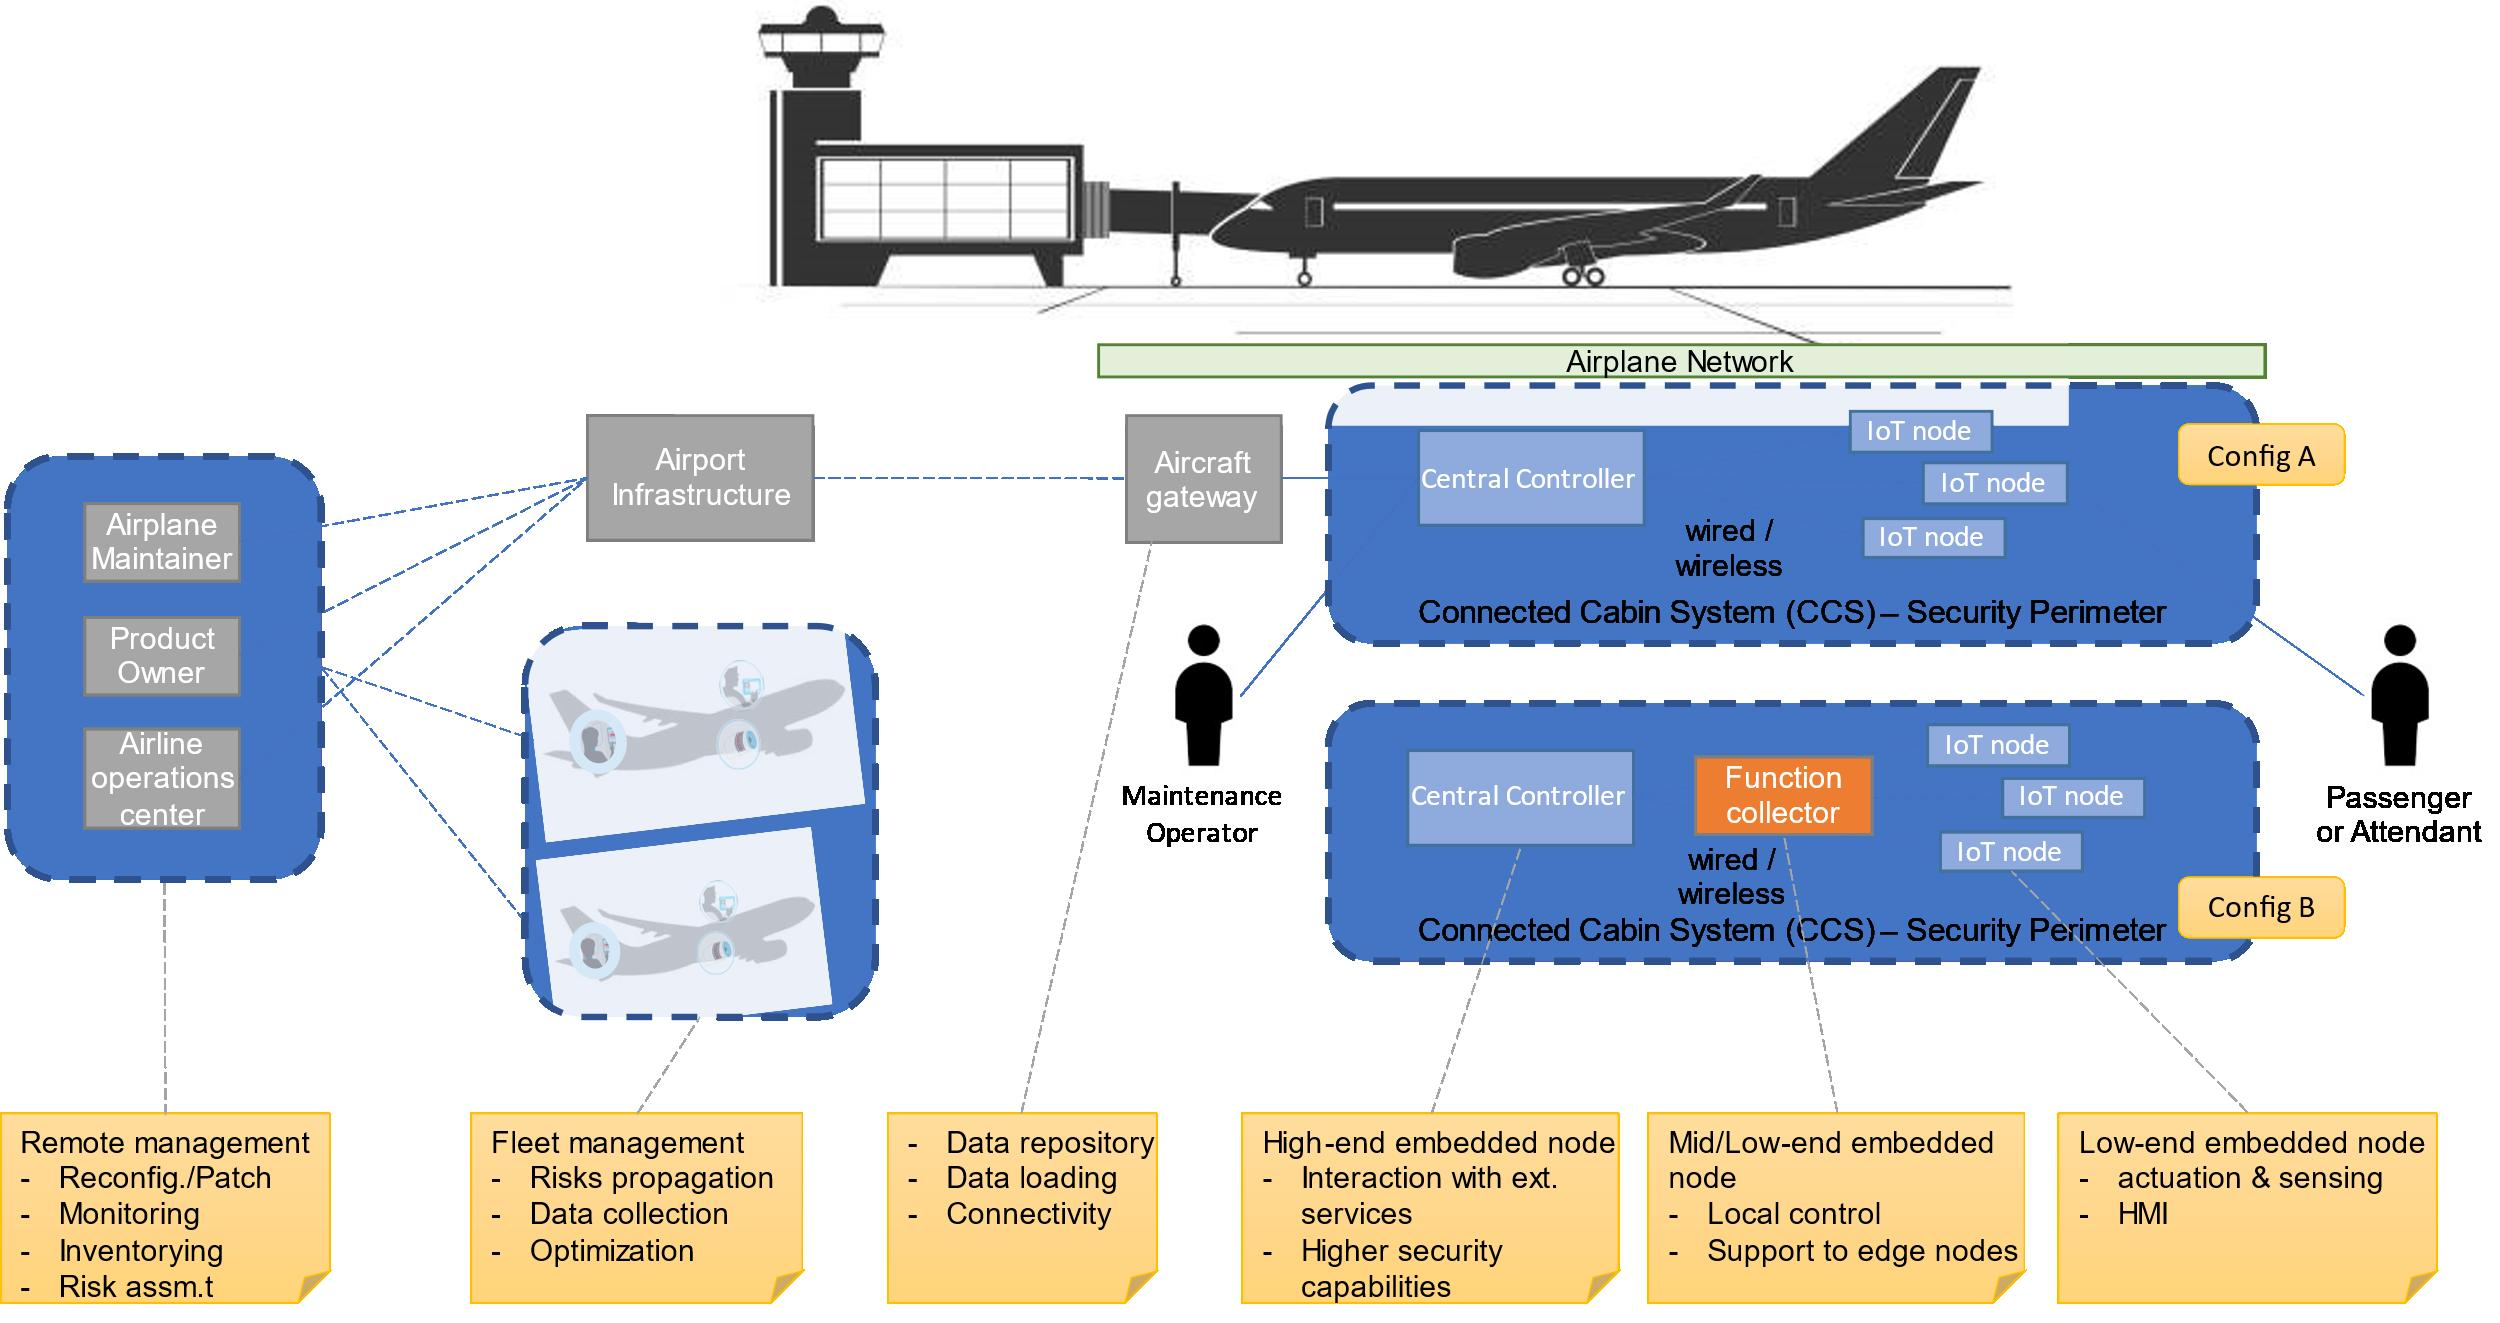
\includegraphics[width=0.95\textwidth]{figures/collins-ccs.jpg}
	\end{center}
	\caption{Collins CCS}
	\label{fig:Collins CCS}
\end{figure}

\section{Background}

Our use case will take the CCS scenario from Figure~\ref{fig:Collins CCS} into consideration and build up on their use cases.

Nowadays more and more IoT devices are being deployed to aircraft cabins to improve passenger experience and airline
operations. Benefits span from remote PHM to reduced maintenance time, while also supporting a
continuous (re)certification process. % TODO: (aver) add source, maybe from certify

\section{Actors}

We will consider following actors for our use case.

\begin{itemize}
	\item Airline:
	      Owns the aircraft and oversees interactions and system operations.
	\item Airplane maintainer: They could be e.g., Airplane manufacturer. Oversees maintenance of the aircraft,
	      including the integration of systems designed by different manufacturers and their configuration.
	\item Product Owner: Oversees design and maintenance of systems deployed in the aircraft on assignment of the
	      airplane maintainer.
	\item Maintenance operator: They work for the airplane maintainer. Their responsibilities include e.g.,
	      the replacement of devices or on-site software upgrades of e.g., portable data loaders.
	\item Passenger, Attendant, Pilot: They interact with the aircraft through sensors, actuators or HMI.
\end{itemize}

\section{System Components}

We will consider an aircraft to have multiple networks, covering various aspects.
\begin{itemize}
	\item In-flight entertainment system
	\item Aircraft System
	\item Flight Maintenance
\end{itemize}

For our use case we will assume config 'A' as the main configuration of the networks, where edge nodes are connected to
a central controller that manages the edge nodes as a subnet.
\begin{itemize}
	\item IoT / Edge Nodes: low-end devices, including actuation, sensing or HMI capabilities, with limited
	      room for hardware and software based cybersecurity, that requires offloading to a more capable
	      instance.
	\item Central Controller: High-end devices with ability to host full-fledged security functionalities.
\end{itemize}

External communication will take place through aircraft gateway offering services for data repository, data loading and
connectivity with external environment. The airline operations center, product owner and airplane maintainer can interact
through the airport infrastructure. A technician may directly access the aircraft if necessary.


\section{Scenarios}

\subsection{Installation of Connected Cabin Systems} % (fold)
\label{sub:Installation of Connected Cabin Systems}

\subsubsection{Goals}

The goals of this scenario include bootstrapping and customization of devices for specific deployment, updating and
decommissioning of previous systems, guaranteeing a reset to a known and fresh, wiped data, state.
Table~\ref{tab:Actors involved} highlights the involved actors and Table~\ref{tab:Lifecycle stages involved} shows the
stages involved in this scenario.

\begin{table}
	\caption{Actors involved}
	\label{tab:Actors involved}
	\begin{center}
		\begin{tabular}{ |p{2.5cm}|p{2.5cm}|p{2.5cm}|p{2.5cm}|p{2.5cm}| }
			\hline
			Airline & Airplane Maintainer & Product Owner & Maintenance Operator & Passenger, Attendant, Pilot \\
			\hline
			X       & -                   & X             & -                    & X                           \\
			\hline
		\end{tabular}
	\end{center}
\end{table}

\begin{table}
	\caption{Lifecycle stages involved}
	\label{tab:Lifecycle stages involved}
	\begin{center}
		\begin{tabular}{ |c|c|c|c|c| }
			\hline
			Bootstrapping & Operation & Update & Repurposing & Decommissioning \\
			\hline
			X             & -         & X      & -           & X               \\
			\hline
		\end{tabular}
	\end{center}
\end{table}

\subsubsection{Pre-condition}

In order for this scenario to be valid, following pre-conditions need to be met:
\begin{itemize}
	\item Actors involved can establish a secure connection with the aircraft, wireless or wired, through airport
	      infrastructure
	\item Airport and Aircraft network infrastructure can receive authorization requests for needed connections from
	      the external environment.
	\item The Maintenance Operator is provided access to the airplane and to maintenance ports of the target CCS.

\end{itemize}

\subsubsection{Sub-Scenario 1: Component Installation}

\begin{figure}
	\begin{center}
		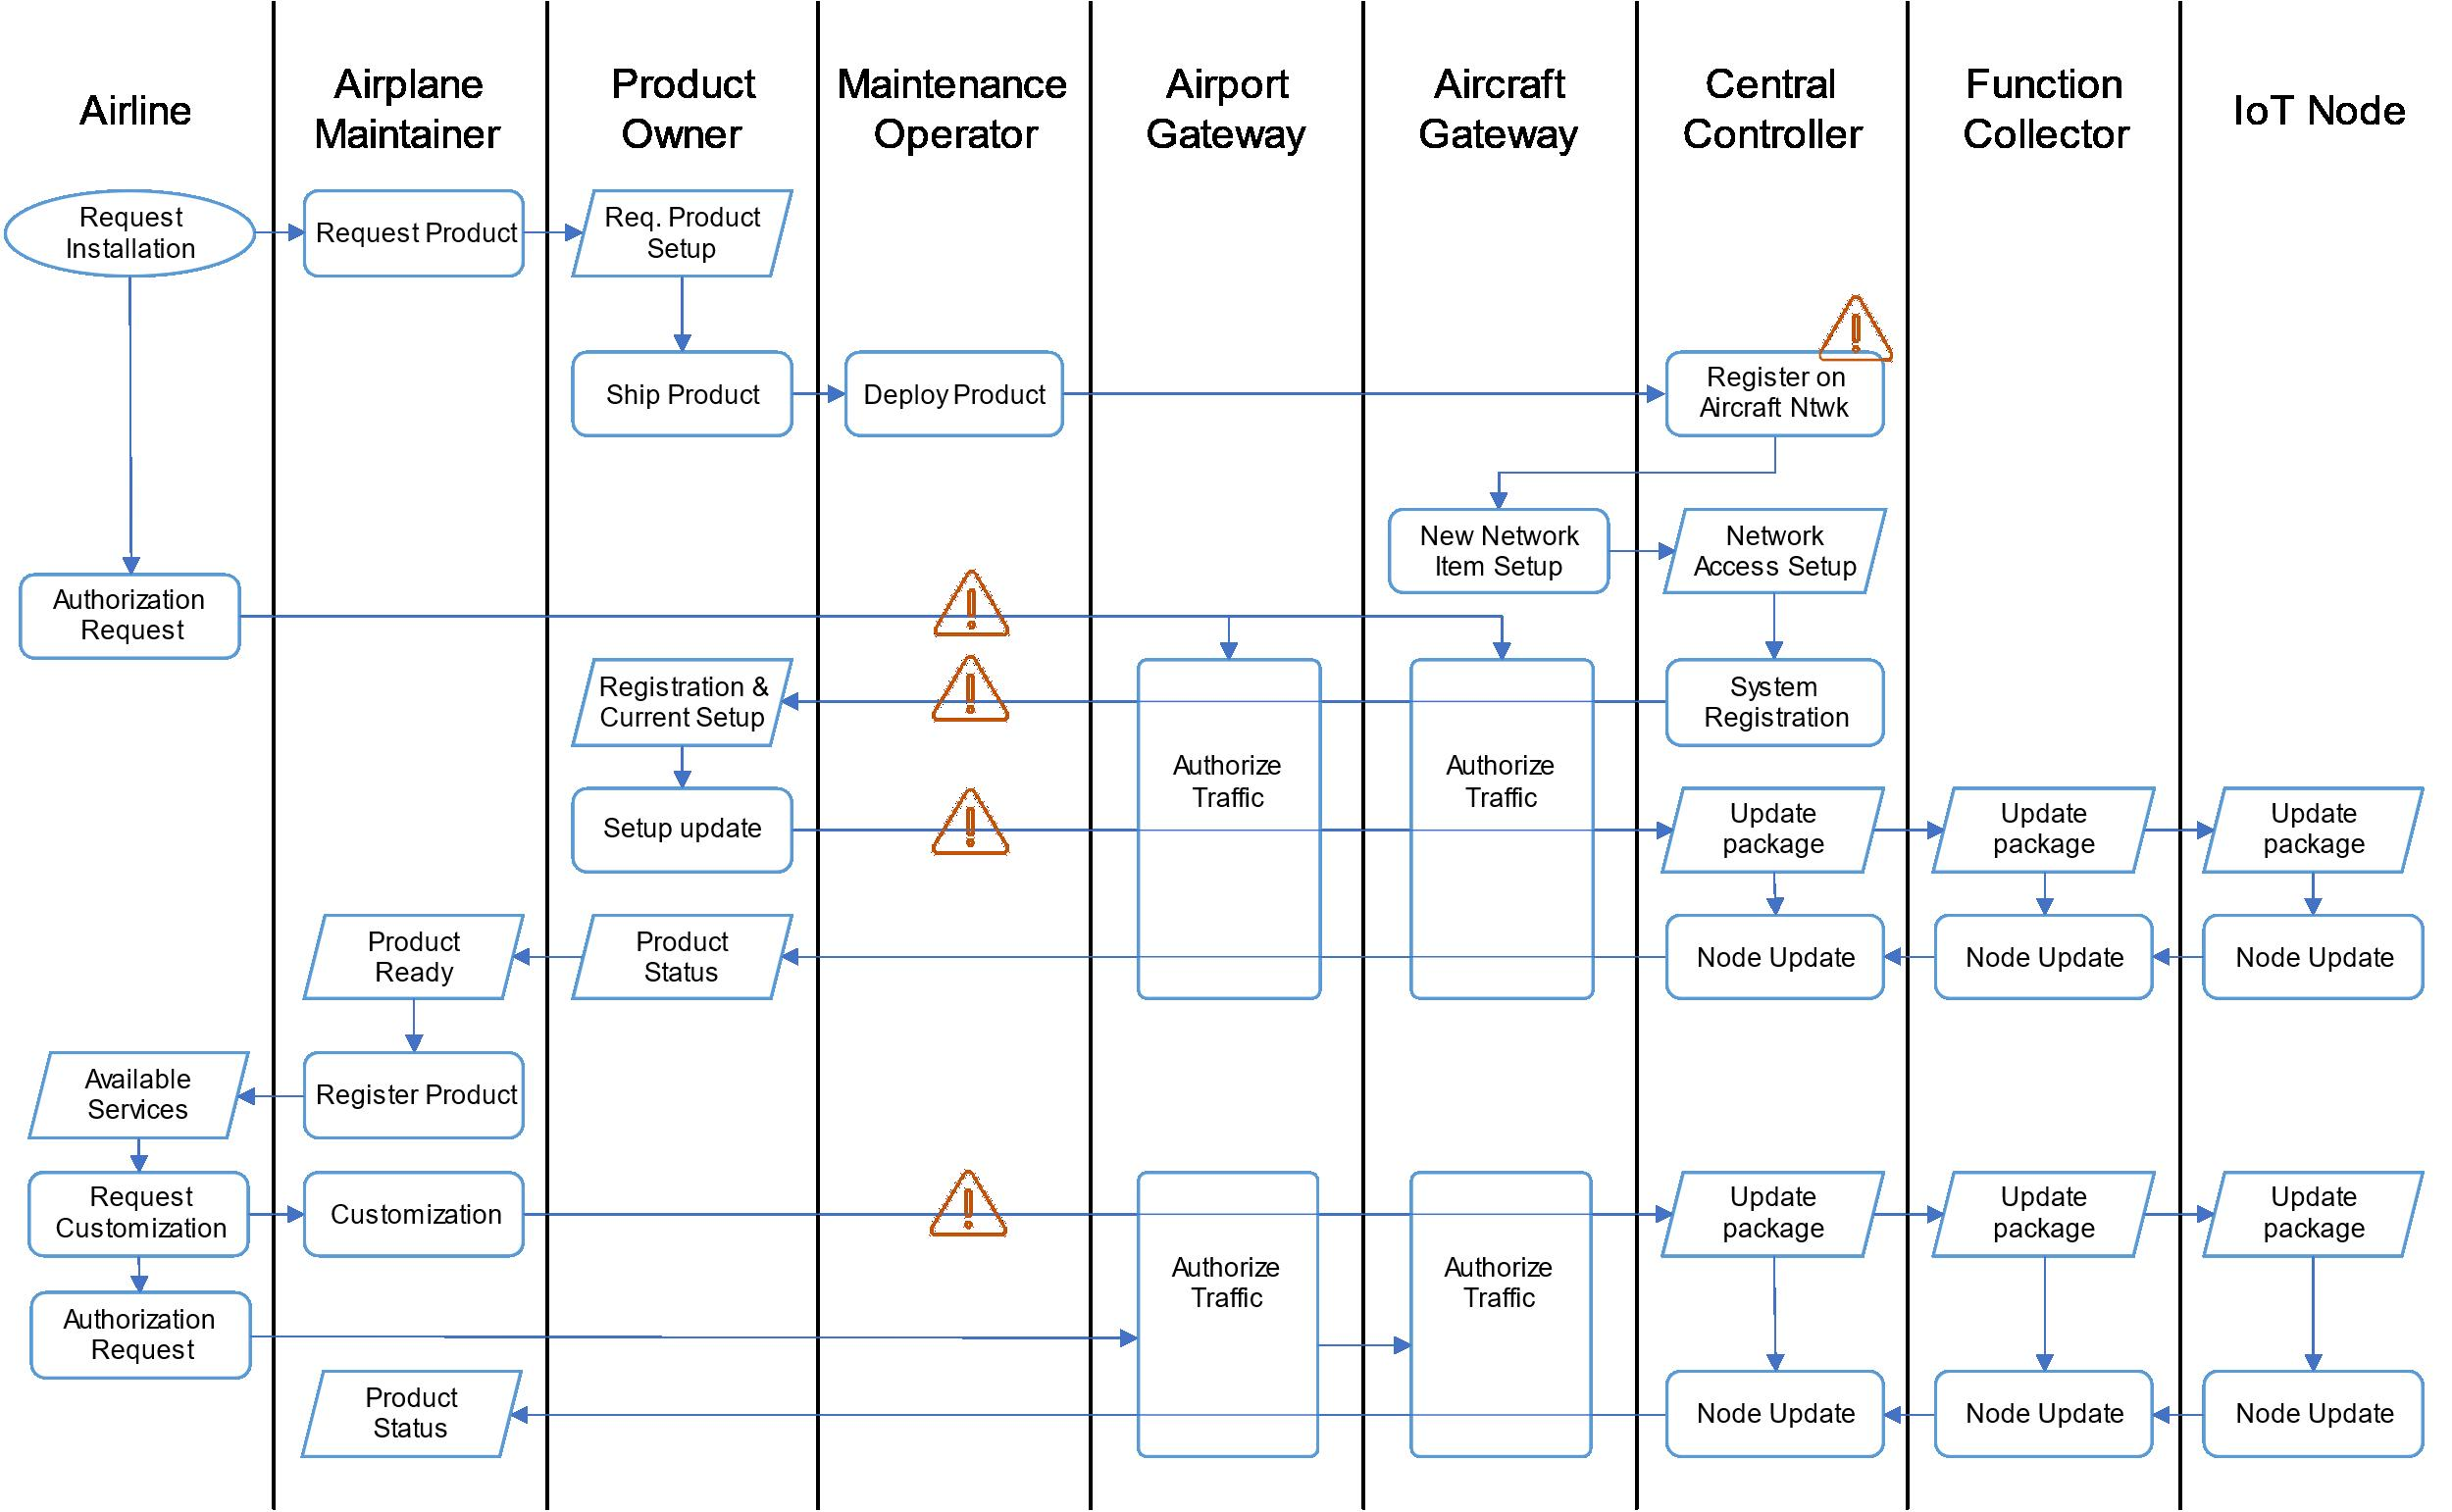
\includegraphics[width=0.95\textwidth]{figures/collins-s1-installation.jpg}
	\end{center}
	\caption{Collins Scenario 1 Installation}
	\label{fig:collins-s1-installation}
\end{figure}

\paragraph{Flow of Events}

The flow of events can be tracked in Figure~\ref{fig:collins-s1-installation} and is verbalized as follows:

\begin{itemize}
	\item Airline requests installation of new component to the Airplane Maintainer also issuing an authorization
	      request to Airport and Airplane gateways
	\item The request is forwarded to the Product Owner and then to the Maintenance Operator, who oversees the
	      physical deployment of the product.
	\item Once connected, Central Controller registers on the Aircraft Network and receives required setup to
	      complete network access and system registration.
	\item Product Owner is now able to reach the CCS, push configuration and security updates to the Central
	      Controller, as well as the Function Collector and IoT nodes.
	\item After the update, the product is registered and the Airplane Maintainer can offer remote services to the
	      Airline
	\item The Airline requests a customization of the CCS. It is performed by the Airplane Maintainer by pushing an
	      update package and/or modifying specific configurations as allowed by the Product Owner API for
	      Maintenance.
	\item The new product status is confirmed with a feedback message.
\end{itemize}

\subsubsection{Sub-Scenario 2: Component Replacement}

\begin{figure}
	\begin{center}
		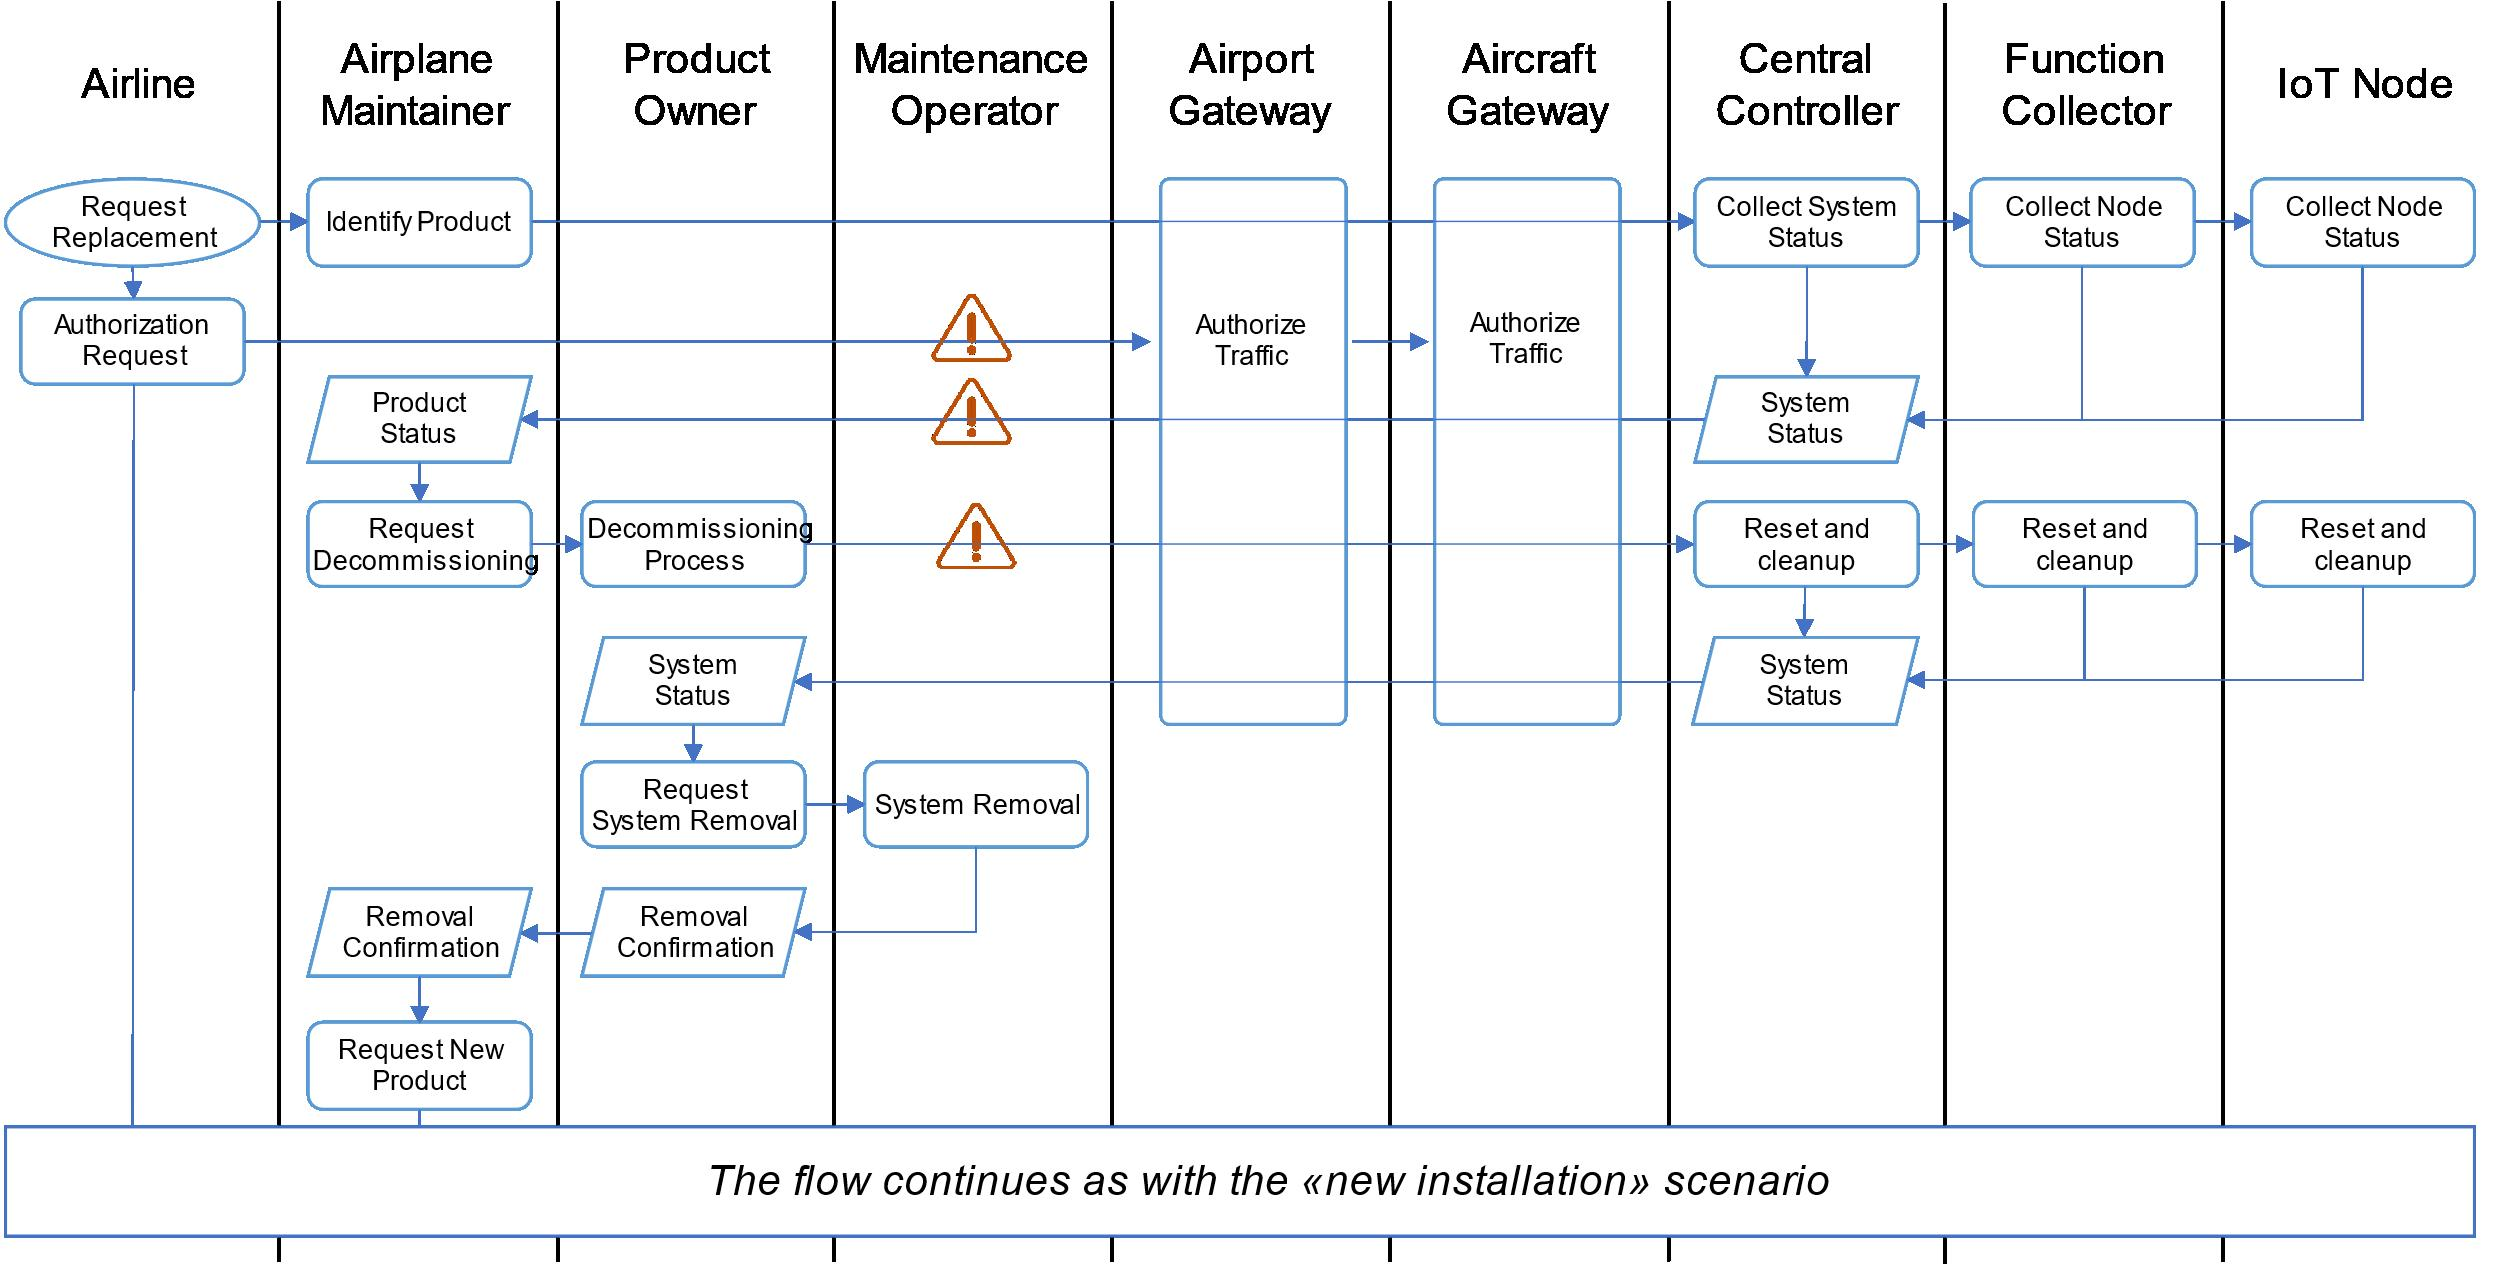
\includegraphics[width=0.95\textwidth]{figures/collins-s1-replacement.jpg}
	\end{center}
	\caption{Collins Scenario 1 Replacement}
	\label{fig:collins-s1-replacement}
\end{figure}

\paragraph{Flow of Events}

\begin{itemize}
	\item Airline requests replacement of a component to the Airplane maintainer, also issuing an authorization
	      request to the Airport and Airplane Gateways
	\item The Airplane Maintainer identifies the target product (location) and collects latest system status.
	\item The Airplane Maintainer issues a decommissioning request to the Product Owner and starts the
	      decommissioning process, which causes a reset and cleanup of all the nodes that will be replaced
	\item After remote reset and clean-up, product owner requests the Maintenance Operator to physically remove the
	      system from the cabin.
	\item The product is then unregistered and can be dismissed.
	\item The remaining part continues with the 'New installation process flow'
\end{itemize}

\subsubsection{Post-Condition}

After completion of the Installation Scenario, following post-conditions need to be met:

\begin{itemize}
	\item New component is deployed in the CCS, integrated into the network, updated with latest security patches
	      and configured by the Airline for their specific needs.
	\item Component is securely onboarded in the CCS, unique identity and certificates are dispatched for
	      authentication.
\end{itemize}

\subsubsection{Attack Scenario}

As an alternative flow of events, i.e., in an attack scenario, highlighted by the yellow triangles in
Figure~\ref{fig:collins-s1-installation} and Figure~\ref{fig:collins-s1-replacement} following points were identified:

\begin{itemize}
	\item Attacker can inject malicious payloads in place of the intended one, (confidential) credentials provided
	      to the Central Controller for network access and authentication ca be stolen.
	\item IP sensitive data can be lead by the Airplane Maintainer when retrieving system status
	\item maintenance/reset/cleanup procedures integrity can be compromised
\end{itemize}

% subsection Installation of Connected Cabin Systems (end)

\subsection{System Operation and Monitoring}
